\documentclass{article}

\usepackage[english]{babel}
\usepackage[letterpaper,top=3cm,bottom=2.5cm,left=2.5cm,right=2.5cm,marginparwidth=1.75cm]{geometry}
\usepackage{amsmath, amssymb, graphicx, multicol, bm, booktabs, tabularx, fancyhdr}
\usepackage[colorlinks=true, allcolors=blue]{hyperref}

\pagestyle{fancy}
\fancyhf{}
\rhead{Jacob Sigman\\3/31/22}
\lhead{MA-240-A\\Ordinary and Partial Differential Equations}
\cfoot{\thepage}
\renewcommand{\headrulewidth}{1.5pt}

\title{MA-240-A Midterm Exam Corrections}
\author{Jacob Sigman}
\date{3/31/22}

\begin{document}
\maketitle
\newpage
\tableofcontents
\newpage
\section*{Question 1}
\addcontentsline{toc}{part}{Question 1}
\begin{enumerate}
    \item \textbf{False} - Use the Wronskian to determine if a \(S\) is linearly independent. If the Wronskian is 0, then \(S\) is linearly dependent. Since \(f=0\in S\), this makes the Wronskian 0, since the whole column of the Wronskian is 0, therefore \(S\) is linearly dependent.
    \item \textbf{False} - The leading term for a critically damped oscillator is \(te^{-t}\), but for an overdamped oscillator the leading term is \(e^{-t+b}\) which will cause the oscillator to move in the other direction, making it's approach to 0 slower.
    \item \textbf{False} - Solutions are not defined as points, but as curves.
    \item \textbf{False}
    \item \textbf{True}
    \item \textbf{True} - Since the derivative of the function is 0 at that point, while it may \underline{touch} the line, it'll never \underline{cross} the line.
    \item \textbf{False} - Some ODEs have solutions that can only be represented visually, so not every ODE would possess an exact solution.
    \item \textbf{True} - A linear homogeneous ODE possesses at least one solution, that solution being 0 (the trivial solution).
\end{enumerate}
\section*{Question 2}
\addcontentsline{toc}{part}{Question 2}
Define a bounded region in the \(xy\)-plane containing the point \((x_0, y_0)\). If \(f(x,y)\) and \(\frac{\partial f}{\partial y}\) are continuous in the region, then there exists an interval \(I\) and a unique function \(y(x)\in I\) that is a solution for this problem.
\section*{Question 3}
\addcontentsline{toc}{part}{Question 3}
\begin{center}
Let \(L\) be the differential operator defined as
\[L=\sum_{n=0}^{k}a_n(x)D^{(n)}\]
This means that:
\[L(y)=g_1(x),\,g_2(x),\,\cdots,\,g_n(x)\]
if and only if the following is defined as the particular solution:
\[y_p=\sum_{j=1}^ky_{p_j}(x)\]
By the superposition principle, the result is:
\[L(y_p)=L\left(\sum_{j=1}^ky_{p_j}(x)\right)=\sum_{j=1}^kL\left(y_{p_j}(x)\right)=\sum_{j=1}^kg_j(x)\]
\end{center}
\section*{Question 4}
\addcontentsline{toc}{part}{Question 4}
\subsection*{Part 1}
\addcontentsline{toc}{section}{Part 1}
\begin{center}
\[3(1+t^2)y'=2ty(y^3-1)\]
\[3(1+t^2)\frac{dy}{dt}=2t(y^4-y)\]
\[\frac{3}{y^4-y}dy=\frac{2t}{1+t^2}dt\]
Perform partial fraction decomposition on \(\frac{3}{y^4-y}\).
\[\frac{3}{y^4-y}=\frac{3}{y(y^3-1)}=\frac{3}{y(y-1)(y^2+y+1)}=-\frac{3}{y}+\frac{1}{y-1}+\frac{Ay+B}{y^2+y+1}\]
\[-\frac{3}{y}+\frac{1}{y-1}+\frac{Ay+B}{y^2+y+1}=3\]
\[-3(y-1)(y^2+y+1)+y(y^2+y+1)+(Ay+B)(y)(y-1)=3\]
\[-3y^3+3+y^3+y^2+y+Ay^3-Ay^2+By^2-By=3\]
\[Ay^3-3y^3+y^3=0\hspace{7 mm}A=2\]
\[y-By=0\hspace{7 mm}B=1\]
\[\frac{3}{y^4-y}=-\frac{3}{y}+\frac{1}{y-1}+\frac{2y+1}{y^2+y+1}\]
Substitute partial fraction decomposition into seperable equations.
\[\int\left[-\frac{3}{y}+\frac{1}{y-1}+\frac{2y+1}{y^2+y+1}\right]dy=\int\frac{2t}{1+t^2}dt\]
\[\int\left[-\frac{3}{y}+\frac{1}{y-1}+\frac{2y+1}{y^2+y+1}\right]dy=-3\ln|y|+\ln|y-1|+\ln|y^2+y+1|\]
\[\int\frac{2t}{1+t^2}dt=\ln|1+t^2|+c\]
\[-3\ln|y|+\ln|y-1|+\ln|y^2+y+1|=\ln|1+t^2|+c\]
\[\boxed{y=\frac{1}{\sqrt[3]{-e^ct^2-e^c+1}}\hspace{3 mm}t\in{\rm I\!R}}\]
\end{center}
\newpage
\subsection*{Part 2}
\addcontentsline{toc}{section}{Part 2}
\[y^{(5)}-9y^{(4)}-y^{(3)}-8y''-90y'=-\sin(3x)\]
\[\textnormal{Auxillary Equation: }m^5-9m^4-m^3-81m^2-90m=0\]
\[m(m-1)(m+10)(m-3i)(m+3i)=0\hspace{7 mm}m=0,\,1,\,-10,\,\pm\sqrt{3}i\]
\[y_c=c_1+c_2e^x+c_3e^{-10x}+c_4\sin\left(\sqrt{3}x\right)+c_5\cos\left(\sqrt{3}x\right)\]
\[\textnormal{Guess: }y_p=Ax\sin(3x)+Bx\cos(3x)\]
\[y_p'=-3Bx\sin(3x)+A\sin(3x)+3Ax\cos(3x)+B\cos(3x)=(A-3Bx)\sin(3x)+(3Ax+B)\cos(3x)\]
\[y_p''=-3(3Ax+B)\sin(3x)-3B\sin(3x)+3(A-3Bx)\cos(3x)+3A\cos(3x)=(-9Ax-6B)\sin(3x)+(6A-9Bx)\cos(3x)\]
\[y_p^{(3)}=-3(6A-9Bx)\sin(3x)-9A\sin(3x)+3(-9Ax-6B)\cos(3x)-9B\cos(3x)\]
\[y_p^{(3)}=(-27A+27Bx)\sin(3x)+(-27Ax-27B)\cos(3x)\]
\[y_p^{(4)}=(81Ax+81B)\sin(3x)+27B\sin(3x)+(81Bx-81A)\cos(3x)-21A\cos(3x)\]
\[y_p^{(4)}=(81Ax+108B)\sin(3x)+(81Bx-108A)\cos(3x)\]
\[y_p^{(5)}=-3(81Bx-108A)\sin(3x)+81A\sin(3x)+3(81Ax+108B)\cos(3x)+81B\cos(3x)\]
\[y_p^{(5)}=(405A-243Bx)\sin(3x)+(243Ax+405B)\cos(3x)\]
\[405A+27A-90A+48B-972B=-1\hspace{7 mm}342A-924B=-1\]
\[405B+27B-90B-48A+972A=0\hspace{7 mm}342B+924A=0\]
\[A=-\frac{342}{924}B\hspace{7 mm}B=\frac{77}{80895}\]
\[A=-\frac{342}{924}B\hspace{7 mm}A=-\frac{26334}{74744208}\]
\[\boxed{y=c_1+c_2e^x+c_3e^{-10x}+c_4\sin\left(\sqrt{3}x\right)+c_5\cos\left(\sqrt{3}x\right)-\frac{26334x}{74744208}\sin(3x)+\frac{77x}{80895}\cos(3x)\hspace{3 mm}x\in{\rm I\!R}}\]
\subsection*{Part 3}
\addcontentsline{toc}{section}{Part 3}
\[y'=\frac{y}{e^{-y}\sin(2y)-(1+y)x}\]
\[\frac{dy}{dx}=\frac{y}{e^{-y}\sin(2y)-(1+y)x}\]
\[\frac{dx}{dy}=\frac{e^{-y}\sin(2y)-(1+y)x}{y}=\frac{-y-1}{y}x+\frac{e^{-y}}{y}\sin(2y)\]
\[\frac{dx}{dy}+\frac{y+1}{y}x=\frac{e^{-y}}{y}\sin(2y)\]
\[\mu=e^{\int\frac{y+1}{y}dy}=ye^y\]
\[\frac{d}{dy}\left[xye^y\right]=\frac{e^{-y}}{y}\sin(2y)\,ye^y=\sin(2y)\]
\[xye^y=-\frac{1}{2}\cos(2y)+c\]
\[\boxed{x=-\frac{1}{2ye^y}\cos(2y)+\frac{c}{ye^y}\hspace{3 mm}y\in(0,\infty)}\]
\subsection*{Part 4}
\addcontentsline{toc}{section}{Part 4}
\[y'=\frac{1+\ln(x)+\frac{y}{x}}{1-\ln(x)}\]
\[\frac{dy}{dx}(1-\ln(x))=1+\ln(x)+\frac{y}{x}\]
\[(1-\ln(x))dy=\left(1+\ln(x)+\frac{y}{x}\right)dx\]
\[\left(1+\ln(x)+\frac{y}{x}\right)dx-(1-\ln(x))dy=0\]
\[\textnormal{Let } \textbf{M}=1+\ln(x)+\frac{y}{x} \textnormal{ and } \textbf{N}=1-\ln(x)\]
\[\textbf{M}_y=\textbf{N}_x=-\frac{1}{x}\]
\[\int\textbf{N}dy=y-y\ln|x|\hspace{7 mm}\int\textbf{M}dx=-x-x\ln|x|+x-y\ln|x|=-x\ln|x|-y\ln|x|\]
\[y-y\ln|x|-x\ln|x|=c\]
\[y(1-\ln|x|)-x\ln|x|=c\]
\[\boxed{y=\frac{c\,x\ln|x|}{1-\ln|x|}\hspace{3 mm}x\in(e,\infty)}\]
\subsection*{Part 5}
\addcontentsline{toc}{section}{Part 5}
\[y'=5-3y+\frac{1}{2}e^{-3x}\]
\[y'+3y=5+\frac{1}{2}e^{-3x}\]
\[\mu=e^{3x}\hspace{7 mm}\frac{d}{dx}\left[e^{3x}y\right]=5e^{3x}+\frac{1}{2}\]
\[e^{3x}y=\frac{5}{3}e^{3x}+\frac{x}{2}+c\]
\[\boxed{y=\frac{5}{3}+\frac{x}{2}e^{-3x}+ce^{-3x}\hspace{3 mm}x\in{\rm I\!R}}\]
\subsection*{Part 6}
\addcontentsline{toc}{section}{Part 6}
\[x^3y^{(3)}-6y=0\]
\[\textnormal{Auxillary Equation: }1(m-2)(m-1)m-6=0\]
\[m^3-3m^2+2m-6=0\]
\[(m-3)(m+2i)(m-2i)=0\hspace{7 mm}m=3,\,\pm\sqrt{2}i\]
\[\boxed{y_c=c_1x^3+c_2\cos\left(\sqrt{2}\ln|x|\right)+c_3\sin\left(\sqrt{2}\ln|x|\right)\hspace{3 mm}x\in(0,\infty)}\]
\newpage
\section*{Question 5}
\addcontentsline{toc}{part}{Question 5}
\begin{center}
\[y'=\sin(x)\cos(y)\]
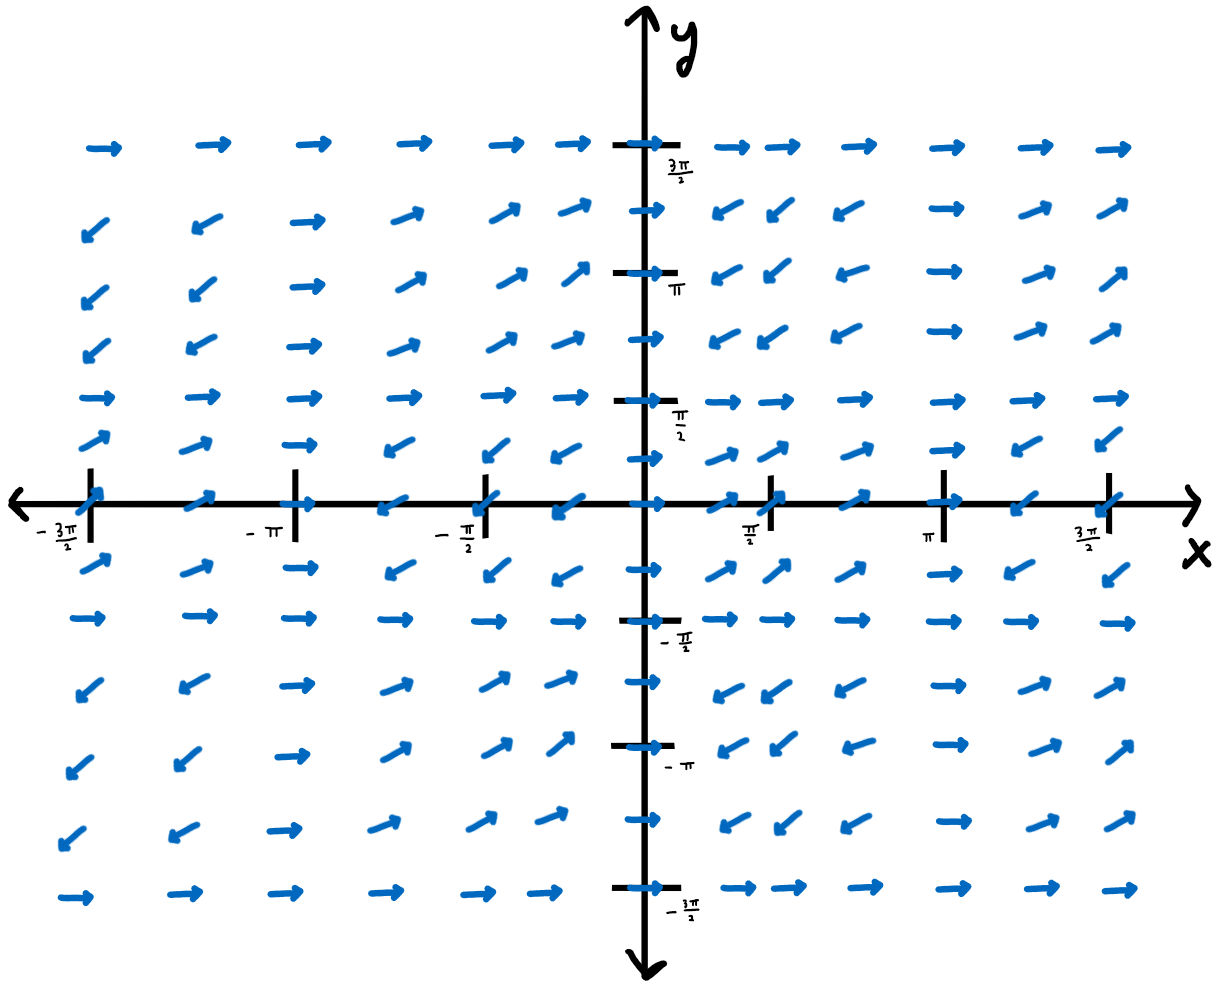
\includegraphics[scale=0.5]{question2.png}
\end{center}
\section*{Question 6}
\addcontentsline{toc}{part}{Question 6}
\[m=1 \textnormal{ kg}\hspace{7 mm}F=kx\hspace{7 mm}k=10\]
\[\frac{d^2x}{dt^2}+8\frac{dx}{dt}+10x=F(t)\]
\[\textnormal{Auxillary Equation: }m^2+8m+10=0\hspace{7 mm}m=\frac{-8\pm\sqrt{64-40}}{2}=-4\pm\sqrt{6}\]
\[x_c=c_1e^{\left(-4+\sqrt{6}\right)t}+c_2e^{\left(-4-\sqrt{6}\right)t}\]
\begin{center}
All terms of the complementary solution are transient.
\end{center}
\subsection*{Part (a)}
\addcontentsline{toc}{section}{Part (a)}
\[\textnormal{Guess: }x_p=A\sin(4t)+B\cos(4t)\]
\[x_p'=4A\cos(4t)-4B\sin(4t)\]
\[x_p''=-16A\sin(4t)-16B\cos(4t)\]
\[-16A-32B+10A=F_0\]
\[-16B+32A+10B=0\]
\[A=\frac{6}{32}B\hspace{7 mm}-16\frac{6}{32}B-32B-\frac{6}{32}B*10=F_0\hspace{7 mm}B=-\frac{8F_0}{265}\hspace{7 mm}A=-\frac{3F_0}{530}\]
\[\boxed{x=c_1e^{\left(-4+\sqrt{6}\right)t}+c_2e^{\left(-4-\sqrt{6}\right)t}-\frac{3F_0}{530}\sin(4t)-\frac{8F_0}{265}\cos(4t)\hspace{3 mm}t\in{\rm I\!R}}\]
\begin{center}
Only the complementary solution is transient.
\end{center}
\subsection*{Part (b)}
\addcontentsline{toc}{section}{Part (b)}
\[\textnormal{Guess: }x_p=Ae^{-4t}\sin(4t)+Be^{-4t}\cos(4t)\]
\[x_p'=4Ae^{-4t}\cos(4t)-4Ae^{-4t}\sin(4t)-4Be^{-4t}\sin(4t)-4Be^{-4t}\cos(4t)\]
\[x_p''=\frac{d}{dt}\left[4Ae^{-4t}\cos(4t)-4Ae^{-4t}\sin(4t)-4Be^{-4t}\sin(4t)-4Be^{-4t}\cos(4t)\right]\]
\[x_p''=\frac{d}{dt}\left[-4e^{-4t}((B+A)\sin(4t)+(B-A)\cos(4t))\right]\]
\[x_p''=16e^{-4t}((B+A)\sin(4t)+(B-A)\cos(4t))-4e^{-4t}(4(B+A)\cos(4t)-4(B-A)\sin(4t))\]
\[x_p''=32Be^{-4t}\sin(4t)-32Ae^{-4t}\cos(4t)\]
\[32B-32A-32B+10A=F_0\]
\[-32A+32A-32B+10B=0\]
\[A=-\frac{F_0}{22}\hspace{7 mm}B=0\]
\[\boxed{x=c_1e^{\left(-4+\sqrt{6}\right)t}+c_2e^{\left(-4-\sqrt{6}\right)t}-\frac{F_0}{22}e^{-4t}\sin(4t)\hspace{3 mm}t\in{\rm I\!R}}\]
\begin{center}
Both the complementary and particular solutions are transient.
\end{center}
\subsection*{Part (c)}
\addcontentsline{toc}{section}{Part (c)}
\[\textnormal{Guess: }x_p=Ae^{-4t}\sin\left(\sqrt{10}t\right)+Be^{-4t}\cos\left(\sqrt{10}t\right)\]
\[x_p'=\sqrt{10}Ae^{-4t}\cos\left(\sqrt{10}t\right)-4Ae^{-4t}\sin\left(\sqrt{10}t\right)-\sqrt{10}Be^{-4t}\sin\left(\sqrt{10}t\right)-4Be^{-4t}\cos\left(\sqrt{10}t\right)\]
\[x_p''=\frac{d}{dt}\left[\sqrt{10}Ae^{-4t}\cos\left(\sqrt{10}t\right)-4Ae^{-4t}\sin\left(\sqrt{10}t\right)-\sqrt{10}Be^{-4t}\sin\left(\sqrt{10}t\right)-4Be^{-4t}\cos\left(\sqrt{10}t\right)\right]\]
\[x_p''=\frac{d}{dt}\left[-e^{-4t}\left(\left(\sqrt{10}B+4A\right)\sin\left(\sqrt{10}t\right)+\left(4B-\sqrt{10}A\right)\cos\left(\sqrt{10}t\right)\right)\right]\]
\begin{center}
\begin{multline*}
x_p''=4e^{-4t}\left(\left(\sqrt{10}B+4A\right)\sin\left(\sqrt{10}t\right)+\left(4B-\sqrt{10}A\right)\cos\left(\sqrt{10}t\right)\right)\\
-e^{-4t}\left(\sqrt{10}\left(\sqrt{10}B+4A\right)\cos\left(\sqrt{10}t\right)-\sqrt{10}\left(4B-\sqrt{10}A\right)\sin\left(\sqrt{10}t\right)\right)
\end{multline*}
\end{center}
\[x_p''=\left(8\sqrt{10}B+6A\right)e^{-4t}\sin\left(\sqrt{10}t\right)+\left(6B-8\sqrt{10}A\right)e^{-4t}\cos\left(\sqrt{10}t\right)\]
\[8\sqrt{10}B+6A-32A-8\sqrt{10}B+10A=F_0\]
\[6B-8\sqrt{10}A+8\sqrt{10}A-32B=0\]
\[A=-\frac{F_0}{16}\hspace{7 mm}B=0\]
\[\boxed{x=c_1e^{\left(-4+\sqrt{6}\right)t}+c_2e^{\left(-4-\sqrt{6}\right)t}-\frac{F_0}{16}e^{-4t}\sin\left(\sqrt{10}t\right)\hspace{3 mm}t\in{\rm I\!R}}\]
\begin{center}
Both the complementary and particular solutions are transient.
\end{center}
\section*{Question 7}
\addcontentsline{toc}{part}{Question 7}
\subsection*{Part (a)}
\addcontentsline{toc}{section}{Part (a)}
\[y'=\frac{y}{x}\]
\[\frac{1}{y}dy=\frac{1}{x}dx\]
\[\int\frac{1}{y}dy=\int\frac{1}{x}dx\]
\[\ln|y|=\ln|x|+c\]
\[\boxed{y=c\,x\hspace{3 mm}x\in{\rm I\!R}}\]
\subsection*{Part (b)}
\addcontentsline{toc}{section}{Part (b)}
\[-ydx+xdy=0\]
\[-\frac{y}{x^2}dx+\frac{1}{x}dy=0\]
\[\textnormal{Let } \textbf{M}=-\frac{y}{x^2} \textnormal{ and } \textbf{N}=\frac{1}{x}\]
\[\textbf{M}_y=\textbf{N}_x=-\frac{1}{x^2}\]
\[\int\textbf{N}dy=\frac{y}{x}\hspace{7 mm}\int\textbf{M}dx=\frac{y}{x}\]
\[\frac{y}{x}=c\]
\[\boxed{y=c\,x\hspace{3 mm}x\in(0,\infty)}\]
\subsection*{Part (c)}
\addcontentsline{toc}{section}{Part (c)}
\[-ydx+xdy=0\]
\[-\frac{y}{x^2+y^2}dx+\frac{x}{x^2+y^2}dy=0\]
\[\textnormal{Let } \textbf{M}=-\frac{y}{x^2+y^2} \textnormal{ and } \textbf{N}=\frac{x}{x^2+y^2}\]
\[\textbf{M}_y=\textbf{N}_x=-\frac{x^2-y^2}{(x^2+y^2)^2}\]
\[\int\textbf{N}dy=\arctan\left(\frac{y}{x}\right)+g(y)\]
\[\frac{\partial}{\partial x}\left[\arctan\left(\frac{y}{x}\right)+g(y)\right]=-\frac{y}{x^2+y^2}+g'(y)\]
\[g'(y)=0\hspace{7 mm}g(y)=c\]
\[\arctan\left(\frac{y}{x}\right)=c\]
\begin{center}
An approximation for \(\arctan\) can be used as follows:
\end{center}
\[\frac{y}{x}=c\hspace{7 mm}c\in\left(-\frac{\pi}{2},\,\frac{\pi}{2}\right)\]
\[\boxed{y=c\,x\hspace{3 mm}x\in{\rm I\!R}}\]
\subsection*{Part (d)}
The answers to (a), (b), and (c) are the same.
\addcontentsline{toc}{section}{Part (d)}
\section*{Question 8}
\addcontentsline{toc}{part}{Question 8}
\subsection*{Part (a)}
\addcontentsline{toc}{section}{Part (a)}
\begin{center}
Let some function \(f_2\) be a constant multiple \(k\) of some function \(f_1\). The Wronskian of the two functions is as follows:
\[W(f_1,f_2)=
\begin{vmatrix}
	f_1 & f_2 \\
	f_1' & f_2'
\end{vmatrix}
=
\begin{vmatrix}
	f_1 & kf_1 \\
	f_1' & kf_1'
\end{vmatrix}
=k\,f_1f_1'-kf_1f_1'=0\]
Since the Wronskian of the two functions is 0, the functions are linearly dependent.
\end{center}
\subsection*{Part (b)}
\addcontentsline{toc}{section}{Part (b)}
\[\frac{d}{dx}\left(|x|^3\right)=\frac{d}{dx}\left(|x|\,x^2\right)=2x\,|x|+\frac{x^3}{|x|}=\frac{3x^3}{|x|}=3x\,|x|\]
\[W\left(x^3,|x|^3\right)=
\begin{vmatrix}
	x^3 & |x|^3 \\
	3x^2 & 3x\,|x|
\end{vmatrix}
=3x^2|x|^3-3x^4|x|=\boxed{0}\]
\subsection*{Part (c)}
\addcontentsline{toc}{section}{Part (c)}
\end{document}
